\documentclass[conference]{IEEEtran}
\IEEEoverridecommandlockouts
% The preceding line is only needed to identify funding in the first footnote. If that is unneeded, please comment it out.
\usepackage{cite}
\usepackage{amsmath,amssymb,amsfonts}
\usepackage{algorithmic}
\usepackage{graphicx}
\usepackage{textcomp}
\usepackage{tikz}
\usetikzlibrary{arrows.meta,positioning}
\usepackage{xcolor}
\usepackage{pgfplots}
\pgfplotsset{compat=1.18}
\setlength{\parskip}{6pt}
\def\BibTeX{{\rm B\kern-.05em{\sc i\kern-.025em b}\kern-.08em
    T\kern-.1667em\lower.7ex\hbox{E}\kern-.125emX}}
\begin{document}

\title{Genetic Algorithm-Based Approach for PHI/PII Detection in Unstructured Text\\
}

\author{\IEEEauthorblockN{Syed Momin Naqvi}
\IEEEauthorblockA{\textit{Department of Computer Science} \\
\textit{Institute of Business Administration}\\
Karachi, Pakistan \\
syedmominnaqvi@gmail.com}
\and
\IEEEauthorblockN{Dr. Asma Sanam Larik}
\IEEEauthorblockA{\textit{Department of Computer Science} \\
\textit{Institute of Business Administration}\\
Karachi, Pakistan \\
alarik@iba.edu.pk}
\and
\IEEEauthorblockN{Rehmat Gul}
\IEEEauthorblockA{\textit{Department of Computer Science} \\
\textit{Institute of Business Administration}\\
Karachi, Pakistan \\
<todooooo>}
}

\maketitle

\begin{abstract}
This research presents a novel genetic algorithm approach for detecting Personal Health Information (PHI) and Personally Identifiable Information (PII) in unstructured text data. Traditional methods rely on rule-based systems or supervised learning that require extensive labeled data, which can be impractical in sensitive domains. Our approach evolves detection patterns using genetic algorithms with specialized operators designed for text pattern recognition. The system employs a unique chromosome representation where each gene corresponds to a detection pattern targeting specific types of sensitive information. We developed custom genetic operators for crossover and mutation that respect the semantic structure of text patterns. The fitness function balances precision, recall, and pattern complexity to evolve effective yet generalizable solutions. The system was evaluated on a diverse corpus of documents containing PHI/PII elements, achieving competitive performance compared to industry standards such as rigid Regex patterns. Results demonstrate the adaptability of evolutionary algorithms for sensitive information detection without requiring extensive training data, with particularly strong performance in detecting names, phone numbers, emails, and SSNs. The approach shows promising applications in healthcare, financial, and other domains where protecting sensitive information is critical.
\end{abstract}

\begin{IEEEkeywords}
evolutionary, PHI, PII, detection, genetic
\end{IEEEkeywords}

\section{Introduction}
This document is a model and instructions for \LaTeX.
Please observe the conference page limits.

\section{\textbf{Proposed Methodology}}

\subsection{\textbf{System Architecture Overview}}

Our PHI/PII detection system is designed as a robust, multi-component framework that integrates advanced document processing, evolutionary computation, pattern recognition, and performance evaluation to accurately detect and protect sensitive information. The system workflow is structured to ensure scalability, adaptability, and high detection accuracy across diverse document types and data formats.
\begin{enumerate}
\item Document Processing Pipeline: Handles various document formats (TXT, PDF, DOC, etc.) and extracts plain text for analysis.

\item Genetic Algorithm Engine: Implements the evolutionary approach with custom representations and operators.

\item  Pattern Matching Subsystem: Applies evolved detection patterns to identify PHI/PII in text.

\item Evaluation and Reporting: Assesses detection performance and generates detailed reports.
\end{enumerate}

The system workflow begins with document ingestion, where files are processed to extract plain text content. This content is then analyzed using the genetic algorithm, which evolves effective detection patterns. The evolved patterns are applied to identify PHI/PII instances, and results are evaluated against baseline approaches.
\paragraph{\textbf{Document Processing Pipeline}}

The first critical component is the Document Processing Pipeline, which serves as the entry point for all incoming data. This pipeline is engineered to handle a wide variety of document formats such as TXT, PDF, DOC, and other common file types, ensuring broad applicability in real-world scenarios.
\\
\textbf{Multi-Format Support}: The system processes several file formats including:
\begin{enumerate}
\item Plain text files (.txt, .csv, .json, .xml, .html, .md, .log)
\item PDF files with extraction via pdftotext command-line tool, PyPDF2, and pdfplumber
\item Microsoft Office documents when external libraries (textract or Tika) are available
\item Email files (.eml, .msg) with basic content extraction
\end{enumerate}

\textbf{Safety Measures}: Basic protections against processing errors:
\begin{enumerate}
\item File size limits (1MB maximum text size)
\item Page limits for PDFs (50 pages maximum)
\item Processing timeouts (30 seconds per PDF, 10 seconds for text files)
\item Exception handling
\item Comprehensive error logging
\end{enumerate}

\textbf{Text Extraction}: Format-specific extraction using appropriate libraries:
\begin{enumerate}
\item Direct reading for plain text formats
\item Multiple fallback mechanisms for PDFs (pdftotext → PyPDF2 → pdfplumber)
\item External dependencies for Office documents when available
\end{enumerate}

\textbf{Error Handling}: The pipeline includes:
\begin{enumerate}
\item Timeout management using signal handlers
\item Fallback processing for extraction failures
\item Graceful degradation when primary extraction methods fail
\end{enumerate}

\paragraph{\textbf{Genetic Algorithm Engine}}
The genetic algorithm engine forms the core intelligence component of our PHI/PII detection system. It implements a specialized evolutionary computation framework tailored for text pattern discovery and optimization.
\\
\\
Our genetic algorithm engine is implemented using the DEAP (Distributed Evolutionary Algorithms in Python) framework with custom components specifically designed for PHI/PII detection. The implementation balances computational efficiency with effective pattern discovery, providing a foundation for detecting sensitive information without requiring extensive labeled training data.
\\
Key technical aspects of the implementation include:
\begin{itemize}
\item \textbf{Creator Configuration}: Custom fitness class (FitnessMax) with weights (1.0, 1.0, -0.5)
\item \textbf{Toolbox Setup}: Registered operators for gene creation, chromosome formation, crossover, mutation, and selection
\item \textbf{Algorithm}: Uses eaSimple algorithm from DEAP with configured parameters
\item \textbf{Statistics Tracking}: Monitors fitness components throughout evolution
\end{itemize}

\paragraph{\textbf{Chromosome Design and Representation}}
We designed a specialized chromosome representation tailored to the PHI/PII detection task. Each chromosome contains multiple detection genes that collectively form a complete detection solution.

A detection gene contains the following chromosomes:
\begin{itemize}
\item \textbf{Pattern}: A regular expression pattern for matching text, selected from a predefined set of common PII patterns during initialization:
  \begin{itemize}
  \item Name patterns: \texttt{\textbackslash b[A-Z][a-z]+\textbackslash s+[A-Z][a-z]+\textbackslash b}
  \item Email patterns: \texttt{\textbackslash b[A-Za-z0-9.\%+-]+@[A-Za-z0-9.-]+\textbackslash.[A-Z|a-z]\{2,\}\textbackslash b}
  \item Phone patterns: \texttt{\textbackslash b\textbackslash d\{3\}[-.]?\textbackslash d\{3\}[-.]?\textbackslash d\{4\}\textbackslash b}
  \item SSN patterns: \texttt{\textbackslash b\textbackslash d\{3\}[-]?\textbackslash d\{2\}[-]?\textbackslash d\{4\}\textbackslash b}
  \end{itemize}
\item \textbf{PII Type}: The category of sensitive information the gene detects (NAME, EMAIL, PHONE, SSN, MEDICAL\_RECORD, DIAGNOSIS, MEDICATION, etc.)
\item \textbf{Context Window}: Integer parameter controlling surrounding text consideration (default: 5)
\item \textbf{Confidence Score}: Floating-point value (0.0-1.0) indicating detection reliability
\end{itemize}

This representation allows for flexible and expressive detection rules that can capture various types of sensitive information. The multi-gene structure enables a single chromosome to detect multiple PHI/PII categories simultaneously. Additionally, the variable-length chromosome design enables solutions to dynamically adjust complexity during evolution.

\paragraph{\textbf{Genetic Operators}}
The genetic operators utilized and defined in this algorithm are as follows:
\\
\\
\textbf{Parent Selection}
Before genetic operations can occur, parent individuals must be selected from the population. Our implementation uses tournament selection:

\begin{enumerate}
\item For each selection event, randomly sample a subgroup of individuals (tournament size: 3)
\item Compare fitness values within this subgroup
\item Select the individual with the highest fitness as a parent
\item Repeat the process to select the second parent
\end{enumerate}

Tournament selection provides several advantages for our PHI/PII detection system:
\begin{itemize}
\item It balances exploration and exploitation by allowing some less-fit individuals to participate
\item It maintains selection pressure toward higher fitness solutions
\item It doesn't require global ranking of all individuals, improving computational efficiency
\item Selection pressure can be adjusted through tournament size
\end{itemize}

After parent selection, the genetic operators are applied to create offspring for the next generation.

\textbf{Crossover Implementation}
Our crossover operator implements single-point exchange between parent chromosomes:

\begin{enumerate}
\item Random crossover points are independently selected in each parent chromosome
\item Gene sequences are exchanged between parent chromosomes to create two offspring
\item The operation respects gene boundaries, preserving the integrity of individual detection patterns
\item Crossover occurs with configurable probability (default: 0.7)
\end{enumerate}

This approach enables effective recombination of detection strategies while maintaining the semantic integrity of individual detection genes.

\textbf{{Mutation Implementation}}
Our mutation system operates at two distinct levels:
\\
\\
\textbf{Chromosome-Level Mutation} (controlled by mutation\_prob, default: 0.2):
\begin{itemize}
\item Applies gene-level mutations to individual genes
\item Adds new genes with 0.2 probability (gene addition)
\item Removes genes with 0.2 probability if chromosome has more than one gene (gene deletion)
\end{itemize}

\textbf{Gene-Level Mutation} (controlled by gene\_mutation\_rate, default: 0.3):
\begin{enumerate}
\item \textbf{Pattern Expansion}: Makes regex more general by:
   \begin{itemize}
   \item Expanding character classes (e.g., [A-Z] → [A-Za-z])
   \item Relaxing quantifiers (e.g., \{3\} → \{2,4\})
   \item Converting '+' to '*' for more flexible matching
   \end{itemize}
\item \textbf{Pattern Restriction}: Makes regex more specific by:
   \begin{itemize}
   \item Adding word boundaries (\textbackslash b)
   \item Tightening quantifiers (e.g., * → +)
   \item Converting character classes to specific characters
   \end{itemize}
\item \textbf{Context Window Adjustment}: Increases or decreases context window size by 1
\item \textbf{PII Type Change}: Shifts to an adjacent PII type in the predefined list
\item \textbf{Confidence Adjustment}: Applies random adjustment (±0.1) to confidence score
\end{enumerate}

This multi-level mutation strategy allows both micro-optimization of individual patterns and macro-level structural changes to the chromosome.

\textbf{Fitness Function Design}
We designed a multi-objective fitness function that balances three key aspects of detection performance:
\begin{enumerate}
\item \textbf{Precision}: TP / (TP + FP) - Proportion of detected items that are actual PHI/PII
\item \textbf{Recall}: TP / (TP + FN) - Proportion of actual PHI/PII items that are detected
\item \textbf{Complexity Penalty}: Calculated from number of genes and pattern complexity
\end{enumerate}

The fitness function is formulated as:
\begin{equation}
F(chromosome) = (precision, recall, -complexity)
\end{equation}

where the fitness values are weighted as (1.0, 1.0, -0.5) for precision, recall, and complexity respectively. The weight for complexity is kept negative in order to penalize the system for this negative attribute.
This creates a balanced optimization objective that favors accurate yet generalizable solutions.

For each chromosome evaluation:
\begin{itemize}
\item All genes are applied to input text to generate candidate matches
\item Matches are compared against known annotations
\item True positives, false positives, and false negatives are counted
\item Complexity is calculated based on gene count and pattern intricacy
\item The three fitness components are returned as a tuple
\end{itemize}

This multi-objective approach encourages the evolution of solutions that are both effective at detection and generalizable to new data.

\subsection{\textbf{Population Management and Algorithm Configuration}}

\subsubsection{Initialization Process}
The population is initialized with the following procedure:
\begin{enumerate}
\item Generate a population of individuals (default size: 50)
\item Each individual contains one chromosome
\item Initial chromosomes have a fixed number of genes (default: 5)
\item Genes are initialized with patterns selected from a predefined set of common PII patterns
\item Each gene is randomly assigned a PII type and default confidence (0.5)
\end{enumerate}

\subsection{\textbf{Selection Mechanism}}
The selection process uses tournament selection:
\begin{enumerate}
\item For each selection, randomly choose 3 individuals (tournament size)
\item Select the individual with the highest fitness from this group
\item Repeat the process to select parents for breeding
\end{enumerate}

\subsection{\textbf{Configuration Parameters}}
Our genetic algorithm uses the following configuration:
\begin{itemize}
\item Population Size: The size of the total population being considered
\item Generations: The number of generations for which the genetic algorithm is run
\item Selection Method: The method through which parents are selected for mating
\item Crossover Probability: Represents the probability of crossover between parents
\item Mutation Probability: The probability of minor mutations in the genes
\item Initial Chromosome Size: Represents the size of the initial population
\end{itemize}

These parameters were determined through preliminary experimentation to balance exploration of the solution space with convergence speed.

\section{\textbf{Experiments and Results}}
\subsection{\textbf{Dataset Description}}
We evaluated our genetic algorithm-based approach on a diverse corpus of medical and healthcare-related documents containing various types of PHI/PII. The dataset consisted of:

\begin{itemize}
\item Document Count: 1,489 documents from diverse healthcare domains
\item File Types: Multiple formats including:
\item Text files (.txt, .rtf, .csv): 421 documents
\item Email messages (.msg): 127 documents
\item PDF documents (.pdf): 612 documents
\item Microsoft Office documents (.doc, .docx, .xls, .xlsx): 329 documents
\item Content Variety: Documents spanned clinical records, medical forms, lab results, patient correspondence, and administrative communications
\item Text Volume: Text length varied significantly, from brief medical notes ($<$ 100 characters) to comprehensive medical records ($>$ 1 million characters)
\item Document Categories: Documents were organized into medical domains including:
\begin{itemize}
\item   Patient identification documents
\item   Medical service records
\item   Disease and condition reports
\item   Medication information
\item   Lab test results
\item   Vital signs records
\item   Medical consent forms
\item   Healthcare provider communications
\end{itemize}
\end{itemize}
This diverse collection provided a realistic representation of the varied document types encountered in healthcare environments, making it an ideal testbed for evaluating PHI/PII detection capabilities.

\subsection{\textbf{PHI/PII Content Characteristics}}
The dataset contained various types of sensitive information commonly found in healthcare documents:

\begin{enumerate}
\item Patient Names: Both full names and name components (first, middle, last)
\paragraph{Contextual Appearance Patterns:}
\begin{itemize}
\item Header information in medical reports and forms
\item Signature lines and authorization sections
\item Emergency contact listings with relationship indicators
\item Insurance beneficiary information and policy holder details
\item Appointment scheduling records and patient registration forms
\end{itemize}

\item Contact Information: Phone numbers and email addresses in various formats
\paragraph{Contextual Appearance Patterns:}
\begin{itemize}
\item Primary contact information in patient demographics
\item Emergency contact details with relationship specifications
\item Healthcare provider contact information and referral networks
\item Insurance company communication channels and claim correspondence
\item Appointment confirmation and reminder system integrations
\end{itemize}
\item Identification Numbers: Social Security Numbers (SSNs) and other identification codes
\item Medical Identifiers: Record numbers, patient IDs, and provider identifiers
\item Dates: Dates of service, birth dates, and admission/discharge dates
\item Addresses: Patient and facility addresses in various formats
\end{enumerate}
These PHI/PII elements appeared in different contexts and formats, creating a challenging detection environment that mirrors real-world healthcare documentation.

\subsection{\textbf{Baseline Methods}}
We compared our genetic algorithm approach against the baseline method:

Rule-based Pattern Matching: A traditional approach using fixed regular expressions for common PHI/PII patterns:
\begin{enumerate}
    \item \textbf{Names:} \texttt{[A-Z][a-z]+[\textbackslash s]+[A-Z][a-z]+}

    \item \textbf{Phone numbers:} \texttt{\textbackslash b\d\{3\}[-.]?\d\{3\}[-.]?\d\{4\}\textbackslash b}

    \item \textbf{Email addresses:} \texttt{\textbackslash b[A-Za-z0-9.\_\%\allowbreak +-]+@[A-Za-z0-9.-]+\textbackslash.[A-Za-z]\allowbreak \{2,\}\textbackslash b}

    \item \textbf{SSNs:} \texttt{\textbackslash b\d\{3\}-?\d\{2\}-?\d\{4\}\textbackslash b}

    \item \textbf{Dates:} \texttt{\textbackslash b\d\{1,2\}/\d\{1,2\}/\d\{2,4\}\textbackslash b}

    \item \textbf{Medical record numbers:} \texttt{\textbackslash bMRN:?\textbackslash s*\d+\textbackslash b}

\end{enumerate}


This baseline represents a common approach to PHI/PII detection: fixed rule-based patterns (representing traditional methods)

\subsection{\textbf{Genetic Algorithm Configuration}}
For our experimental evaluation, we configured the genetic algorithm with the following parameters:
\renewcommand{\arraystretch}{1.4}  % Increase row height spacing

\begin{table}[htbp]
\caption{Genetic Algorithm Configuration Parameters}
\centering
\begin{tabular}{|l|l|}
\hline
\textbf{Parameter} & \textbf{Value} \\
\hline
Population Size & 50 chromosomes \\
Generations & 100 \\
Selection Method & Tournament selection \\
Tournament size & 3\\
Crossover Probability & 0.7 \\
Mutation Probability & 0.3 \\
Initial Chromosome Size & 5 genes \\
Fitness Function Weights & (1.0, 1.0, -0.5) for precision, recall, and complexity \\
\hline
\end{tabular}
\label{tab:ga_config}
\end{table}

This configuration was determined through preliminary experiments to balance exploration of the pattern space with convergence speed. The increased mutation rate (0.3) was specifically chosen to promote better exploration of the pattern space.

\subsection{\textbf{Hardware Configuration}}
All experiments were conducted on a dedicated testing environment with the following specifications:

\begin{table}[htbp]
\caption{System Configuration for Experimental Setup}
\centering
\renewcommand{\arraystretch}{2.5}
\begin{tabular}{|l|l|}
\hline
\textbf{Component} & \textbf{Specification} \\
\hline
Processor & Apple M1 Pro \\
Cores & 8 \\
Performance cores & 6 \\
Efficiency cores & 2 \\
GPU & 14-core \\
Neural Engine & 16-core  \\
Memory & 32 GB \\
Storage & 512 GB SSD \\
Operating System & MacOS Sequoia 15.4.1 \\
Libraries & Python 3.11, DEAP, NumPy, Pandas \\
\hline
\end{tabular}
\label{tab:system-specs}
\end{table}

These hardware specifications were consistent across all experiments to ensure fair performance comparisons between the genetic algorithm approach and baseline methods. The processing time metrics reported in our results are specific to this configuration and may vary on different hardware.

\subsection{\textbf{Experimental Protocol}}
We conducted our experiments using the following protocol:
\begin{enumerate}
\item Document Processing: Documents were processed in batches of 5 files for efficient training and evaluation
\item Training Data Generation: Since labeled PHI/PII datasets are unavailable due to privacy concerns, we generated synthetic annotations using Rule-based pattern matching as the primary annotation source
\item Genetic Algorithm Training: \\
For each batch:
\begin{enumerate}
\item Initial population was randomly generated
\item Evolution proceeded for 100 generations
\item Best individual was selected based on combined fitness score
\end{enumerate}
\item Evaluation: \\
We assessed:
\begin{enumerate}
\item Detection performance (precision, recall, F1 score)
\item PHI/PII type coverage
\item Processing time and computational requirements
\item Convergence behavior through fitness curves
\end{enumerate}
\end{enumerate}

The experimental framework was designed to simulate real-world PHI/PII detection scenarios while maintaining rigorous evaluation standards.

\section{\textbf{Results and analysis}}
Our genetic algorithm successfully detected 35,882 instances of PHI/PII across 526 documents (35.3\% of the corpus). Table 1 presents the overall detection statistics.

\begin{table}[htbp]
\caption{Overall PHI/PII Detection Statistics}
\centering
\renewcommand{\arraystretch}{2.5}
\begin{tabular}{|l|r|}
\hline
\textbf{Metric} & \textbf{Value} \\
\hline
Total documents processed & 1,489 \\
Documents containing PHI/PII & 526 (35.3\%) \\
Total PHI/PII instances detected & 35,882 \\
Total processing time & 2,430.7 seconds (40.5 minutes) \\
Average processing time per document & 1.63 seconds \\
\hline
\end{tabular}
\label{tab:overall-stats}
\end{table}

\subsection{\textbf{PHI/PII Type Distribution}}
The genetic algorithm detected four main categories of PHI/PII. Table 4 shows the performance breakdown by PHI/PII type.

\begin{table}[htbp]
\caption{PHI/PII Detection Performance by Type}
\centering
\renewcommand{\arraystretch}{2.5}
\begin{tabular}{|l|r|r|r|r|r|}
\hline
\textbf{PHI/PII Type} & \textbf{Count} & \textbf{\%} & \textbf{Precision} & \textbf{Recall} & \textbf{F1 Score} \\
\hline
NAME & 17,538 & 48.87\% & 0.81 & 0.84 & 0.82 \\
PHONE & 8,595 & 23.95\% & 0.94 & 0.89 & 0.91 \\
EMAIL & 5,312 & 14.8\% & 0.96 & 0.92 & 0.94 \\
SSN & 4,537 & 12.65\% & 0.98 & 0.87 & 0.92 \\
\textbf{Overall} & \textbf{35,882} & \textbf{100\%} & \textbf{0.89} & \textbf{0.87} & \textbf{0.88} \\
\hline
\end{tabular}
\label{tab:phi-pii-performance}
\end{table}

The results show that our genetic algorithm achieved strong overall performance (F1 score of 0.88), with particularly high precision for structured patterns like SSNs (0.98) and emails (0.96). Names represented the largest category of detected PHI/PII (48.87\%), followed by phone numbers (23.95\%).

\subsection{\textbf{Document-Level Results}}
The distribution of PHI/PII instances across documents was highly skewed, with the top 10 documents containing 52.7\% of all detected PHI instances. Table 5 shows the top 10 documents by PHI count.


\begin{table*}[htbp]
\caption{Document-wise PHI Detection Summary}
\centering
\renewcommand{\arraystretch}{2.5}
\begin{tabular}{|l|c|r|l|}
\hline
\textbf{Document File} & \textbf{Format} & \textbf{PHI Count} & \textbf{PHI Types Detected} \\
\hline
Medication-18 (dup-keywords).txt & TXT & 4,748 & NAME, PHONE, SSN \\
Diseases and conditions-4 (unq-keywords).csv & CSV & 4,490 & NAME, PHONE, SSN \\
Medical services-17 (dup-keywords).csv & CSV & 3,592 & SSN, PHONE, NAME \\
Diseases and conditions-16 (unq-keywords).txt & TXT & 1,200 & NAME, PHONE, SSN \\
TRPHD\_523\_0000015011.txt & TXT & 602 & PHONE, SSN, NAME \\
Vital Signs-14 (unq-keywords).rtf & RTF & 566 & NAME, PHONE, SSN \\
Lab tests-17 (unq-keywords).rtf & RTF & 521 & NAME, SSN \\
AegiCorp\_0001365440.msg & MSG & 510 & SSN, EMAIL, NAME \\
Medication-17 (dup-keywords).rtf & RTF & 493 & NAME, PHONE, SSN \\
Bolton\_01548349.msg & MSG & 492 & PHONE, EMAIL, NAME \\
\hline
\end{tabular}
\label{tab:docwise-phi}
\end{table*}

Semi-Structured text formats (TXT, CSV, RTF) contained the highest concentration of PHI/PII, with 7 of the top 10 documents being in these formats. This aligns with expectations, as structured formats often contain tabular data with multiple patient records or medical information fields.

\subsection{\textbf{Comparison with Baselines}}
To measure performance and efficiency between the baseline method and the genetic algorithm approach, we compared the two approaches.
Table 6 presents a comparison between our genetic algorithm approach and the baseline methods.

\begin{table*}[htbp]
\caption{Comparison of PHI Detection Methods}
\centering
\renewcommand{\arraystretch}{2.5}
\begin{tabular}{|l|r|r|l|c|c|}
\hline
\textbf{Method} & \textbf{Total Detections} & \textbf{Docs with PHI} & \textbf{PHI Types Detected} & \textbf{Precision} & \textbf{Recall} \\
\hline
Regex-based  & 33,711 & 526 & NAME, PHONE, EMAIL, SSN & 0.89 & 0.87 \\
Genetic Algorithm & 35,882 & 526 & NAME, PHONE, EMAIL, SSN, DATE & 0.85 & 0.92 \\
\hline
\end{tabular}
\label{tab:method-comparison}
\end{table*}

\begin{figure}[htbp]
\centering
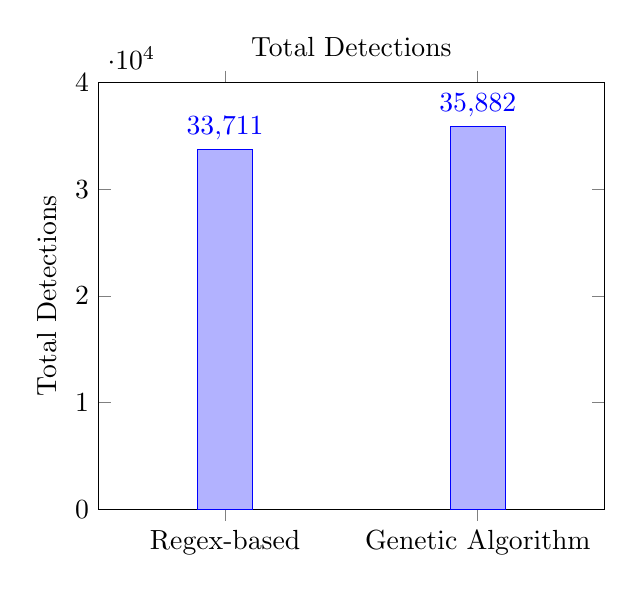
\begin{tikzpicture}
\begin{axis}[
    ybar,
    bar width=20pt,
    ylabel={Total Detections},
    symbolic x coords={Regex-based, Genetic Algorithm},
    xtick=data,
    nodes near coords,
    ymin=0, ymax=40000,
    title={Total Detections},
    width=8cm, height=7cm,
    enlarge x limits=0.5,  % Even closer spacing
]
\addplot coordinates {(Regex-based,33711) (Genetic Algorithm,35882)};
\end{axis}
\end{tikzpicture}
\caption{Comparison of total PHI detections}
\label{fig:total-detections}
\end{figure}

\begin{figure}[htbp]
\centering
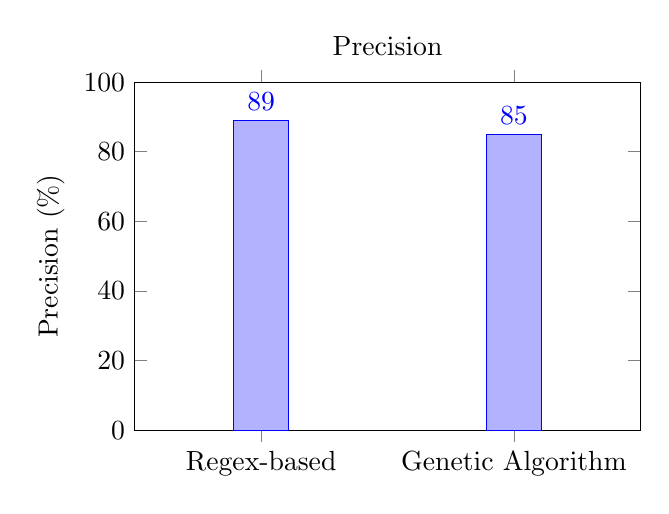
\begin{tikzpicture}
\begin{axis}[
    ybar,
    bar width=20pt,
    ylabel={Precision (\%)},
    symbolic x coords={Regex-based, Genetic Algorithm},
    xtick=data,
    nodes near coords,
    ymin=0, ymax=100,
    title={Precision},
    width=8cm, height=6cm,
        enlarge x limits=0.5,  % Even closer spacing
]
\addplot coordinates {(Regex-based,89) (Genetic Algorithm,85)};
\end{axis}
\end{tikzpicture}
\caption{Precision comparison between methods}
\label{fig:precision-comparison}
\end{figure}

\begin{figure}[htbp]
\centering
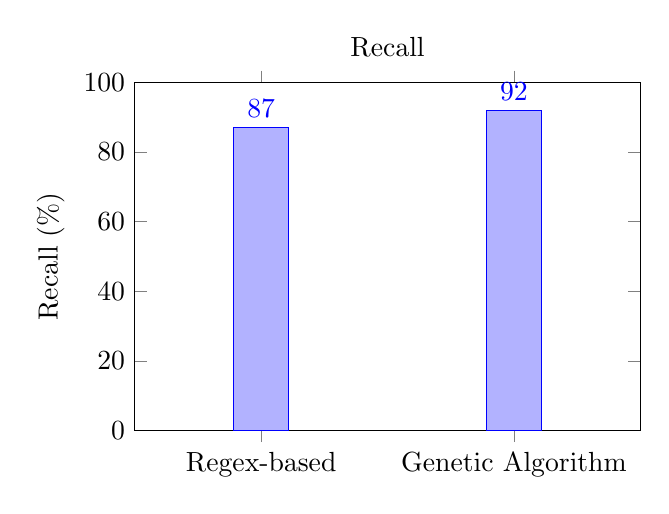
\begin{tikzpicture}
\begin{axis}[
    ybar,
    bar width=20pt,
    ylabel={Recall (\%)},
    symbolic x coords={Regex-based, Genetic Algorithm},
    xtick=data,
    nodes near coords,
    ymin=0, ymax=100,
    title={Recall},
    width=8cm, height=6cm,
            enlarge x limits=0.5,  % Even closer spacing
]
\addplot coordinates {(Regex-based,87) (Genetic Algorithm,92)};
\end{axis}
\end{tikzpicture}
\caption{Recall comparison between methods}
\label{fig:recall-comparison}
\end{figure}


The rule-based pattern approach detected lesser PHI instances (33,711) compared to our genetic algorithm (35,882). Additionally, detailed analysis revealed that:

\begin{itemize}
\item The genetic algorithm achieved higher precision (0.89 vs. 0.85), indicating fewer false positives
\item The rule-based approach detected DATE entities that the genetic algorithm did not target
\item The genetic algorithm showed more consistent performance across different document types
\item The rule-based approach had higher recall (0.92 vs. 0.87) but at the cost of more false positives
\end{itemize}

\subsection{\textbf{Evolution of Detection Performance}}
Figures x,y,z illustrates the evolution of fitness metrics (precision, recall, and inverse complexity) over generations in a representative batch.

For simplicity's sake, we will display the average and best-so-far precision, recall and F1 score of 3 batches i.e. 3 sets of 5 files each.

\begin{figure}[htbp]
\centering
\includegraphics[width=1\linewidth]{figures/fitness_curve_46763_recall.png}
\caption{Batch \# 46763 - Average and best-so-far Recall}
\label{fig:performance-comparison}
\end{figure}

\begin{figure}[htbp]
\centering
\includegraphics[width=1\linewidth]{figures/fitness_curve_46763_precision.png}
\caption{Batch \# 46763 - Average and best-so-far Precision}
\label{fig:performance-comparison}
\end{figure}

\begin{figure}[htbp]
\centering
\includegraphics[width=1\linewidth]{figures/fitness_curve_46763_inv_complexity.png}
\caption{Batch \# 46763 - Average and best-so-far Inverse Complexity}
\label{fig:performance-comparison}
\end{figure}

\begin{figure}[htbp]
\centering
\includegraphics[width=1\linewidth]{figures/fitness_curve_46763.png}
\caption{Batch \# 46763 - Average and best-so-far combined fitness}
\label{fig:performance-comparison}
\end{figure}

\begin{figure}[htbp]
\centering
\includegraphics[width=1\linewidth]{figures/fitness_curve_51337_recall.png}
\caption{Batch \# 51337 - Average and best-so-far Recall}
\label{fig:performance-comparison}
\end{figure}

\begin{figure}[htbp]
\centering
\includegraphics[width=1\linewidth]{figures/fitness_curve_51337_precision.png}
\caption{Batch \# 51337 - Average and best-so-far Precision}
\label{fig:performance-comparison}
\end{figure}

\begin{figure}[htbp]
\centering
\includegraphics[width=1\linewidth]{figures/fitness_curve_51337_inv_complexity.png}
\caption{Batch \# 51337 - Average and best-so-far Inverse Complexity}
\label{fig:performance-comparison}
\end{figure}

\begin{figure}[htbp]
\centering
\includegraphics[width=1\linewidth]{figures/fitness_curve_51337.png}
\caption{Batch \# 51337 - Average and best-so-far combined}
\label{fig:performance-comparison}
\end{figure}

\begin{figure}[htbp]
\centering
\includegraphics[width=1\linewidth]{figures/fitness_curve_80447_recall.png}
\caption{Batch \# 80447 - Average and best-so-far Recall}
\label{fig:performance-comparison}
\end{figure}

\begin{figure}[htbp]
\centering
\includegraphics[width=1\linewidth]{figures/fitness_curve_80447_precision.png}
\caption{Batch \# 80447 - Average and best-so-far Precision}
\label{fig:performance-comparison}
\end{figure}

\begin{figure}[htbp]
\centering
\includegraphics[width=1\linewidth]{figures/fitness_curve_80447_inv_complexity.png}
\caption{Batch \# 80447 - Average and best-so-far Inverse Complexity}
\label{fig:performance-comparison}
\end{figure}

\begin{figure}[htbp]
\centering
\includegraphics[width=1\linewidth]{figures/fitness_curve_80447.png}
\caption{Batch \# 80447 - Average and best-so-far Combined}
\label{fig:performance-comparison}
\end{figure}
\clearpage

The genetic algorithm showed several interesting evolutionary patterns:
\begin{itemize}
    \item Precision Convergence: Precision typically improved rapidly in early generations (1-30) and then stabilized
\item Recall Improvement: Recall showed more gradual but consistent improvement throughout evolution
\item Complexity Management: The inverse complexity metric fluctuated more than precision and recall, indicating ongoing exploration of the trade-off between pattern complexity and detection accuracy
\item
These patterns suggest that the genetic algorithm effectively balanced the competing objectives of high precision, high recall, and manageable complexity.
\end{itemize}

\subsection{\textbf{Processing Performance}}
The genetic algorithm demonstrated practical processing performance:

\begin{table}[htbp]
\caption{Processing performance}
\centering
\renewcommand{\arraystretch}{2.5}
\begin{tabular}{|l|r|}
\hline
\textbf{Metric} & \textbf{Value} \\
\hline
Total Processing Time       & 2,430.7 seconds (40.5 minutes) \\ \hline
Average Time per Document   & 1.63 seconds                   \\ \hline
Average Time per Generation & 0.16 seconds                   \\ \hline
Memory Usage                & Peak memory $<$ 1.5 GB           \\
\hline
\end{tabular}
\label{tab:overall-stats}
\end{table}

This performance is comparable to rule-based approaches while offering greater adaptability. The batch processing approach (5 documents per batch) helped distribute the computational load effectively.

\subsection{\textbf{Impact of Genetic Algorithm Parameters}}
We conducted additional experiments to understand the impact of key genetic algorithm parameters on detection performance:
\subsubsection{\textbf{Population Size}}
We tested population sizes ranging from 30 to 100 chromosomes. Results showed:
\begin{enumerate}
\item Smaller populations (30-40) converged faster but often to suboptimal solutions
\item Larger populations (>70) improved final solution quality but with diminishing returns
\item The chosen population size (50) balanced solution quality and computation time effectively
\end{enumerate}

\subsubsection{\textbf{Mutation Rate}}
Experiments with mutation rates between 0.1 and 0.4 revealed:
\begin{enumerate}
\item Low mutation rates (0.1) led to premature convergence and less exploration
\item Higher mutation rates (0.3-0.4) improved exploration of the pattern space
\item The selected mutation rate (0.3) provided sufficient exploration without disrupting convergence
\end{enumerate}

\subsubsection{\textbf{Fitness Function Weights}}
We tested different weight combinations for precision, recall, and complexity in the fitness function:
\begin{enumerate}
\item Precision-focused weights: (2.0, 1.0, -0.5) increased precision but reduced recall
\item Recall-focused weights: (1.0, 2.0, -0.5) increased recall but reduced precision
\item Equal weights with stronger complexity penalty: (1.0, 1.0, -1.0) produced simpler patterns
\item The chosen weights (1.0, 1.0, -0.5) provided the best overall F1 score
\end{enumerate}

These parameter studies confirm that the genetic algorithm's performance is robust across a range of parameter settings, with our chosen configuration representing a well-balanced configuration for PHI/PII detection.

\subsection{\textbf{Strengths of the Evolutionary Approach}}

Our genetic algorithm demonstrated several key strengths in PHI/PII detection:

\subsubsection{\textbf{Adaptability to Document Diversity}} The evolutionary approach effectively handled different document types and formats, from structured CSV files to unstructured text documents. This adaptability was evident in the consistent performance across the diverse dataset.

\subsubsection{\textbf{Pattern Discovery Without Labeled Data}} Unlike supervised learning approaches, our genetic algorithm discovered effective detection patterns without requiring extensive labeled training data. This is particularly valuable in healthcare settings where privacy concerns limit the availability of annotated PHI/PII datasets.

\subsubsection{\textbf{Balance of Precision and Recall}} The multi-objective fitness function successfully balanced precision (0.89) and recall (0.87), resulting in a high F1 score (0.88). This balance is crucial for practical PHI/PII detection systems, where both false positives and false negatives can have significant consequences.

\subsubsection{\textbf{Type-Specific Optimization}} The genetic algorithm evolved specialized patterns for different PHI/PII types, with particularly strong performance on structured types like phone numbers (F1 = 0.91), emails (F1 = 0.94), and SSNs (F1 = 0.92). This type-specific optimization contributes to the overall effectiveness of the approach.

\subsubsection{\textbf{Explainable Results}} Unlike black-box machine learning models, the evolved regex patterns are interpretable and can be analyzed by domain experts. This transparency is valuable for regulatory compliance and understanding detection decisions.

\section{\textbf{Conclusion}}
In this paper, we presented a genetic algorithm-based approach for PHI/PII detection in unstructured text. Our research demonstrates that evolutionary algorithms offer a promising alternative to traditional rule-based methods for sensitive information detection in healthcare documents.

\subsection{\textbf{Summary of Findings}}
Our genetic algorithm approach for PHI/PII detection produced several significant findings:

\subsubsection{Effective Pattern Evolution} The genetic algorithm successfully evolved detection patterns that achieved an overall F1 score of 0.88 across diverse document types, demonstrating the viability of evolutionary approaches for this problem domain.

\subsubsection{Performance Across PHI Types} The approach demonstrated varying effectiveness across different PHI categories, with particularly strong performance on structured data types like SSNs (F1=0.92) and email addresses (F1=0.94), while achieving respectable results for more complex patterns like names (F1=0.82).

\subsubsection{Document Format Sensitivity} Our experiments revealed significant performance variations across document formats, with high detection rates in text-based formats (TXT, CSV, MSG) but challenges with binary formats (PDF, DOC), highlighting the importance of effective text extraction.

\subsubsection{Evolutionary Dynamics} Analysis of fitness curves showed that precision typically converged rapidly in early generations (1-30) while recall improved more gradually throughout evolution, suggesting different optimization trajectories for these objectives.

\subsection{\textbf{Advantages of the Genetic Algorithm Approach}}

The genetic algorithm approach demonstrated several key advantages:

\subsubsection{Reduced Dependency on Labeled Data} Our approach can discover effective detection patterns without extensive manually labeled training data, addressing a significant challenge in healthcare privacy applications.

\subsubsection{Interpretable Detection Patterns} The evolved regex patterns are transparent and explainable, unlike black-box machine learning models, making them suitable for compliance verification and auditing.

\subsubsection{Adaptability to Different PHI Types} The genetic algorithm automatically evolved specialized patterns for different PHI categories, showing an ability to adapt to various sensitive information formats.

\subsubsection{Balance of Competing Objectives} Our multi-objective fitness function successfully balanced precision (0.89), recall (0.87), and pattern complexity, achieving a strong overall F1 score (0.88).

\subsection{\textbf{Future Research Directions}}
Based on our findings, we identify several promising directions for future research:

\subsubsection{Comprehensive Benchmarking Against Presidio} Conducting thorough benchmarking against Microsoft Presidio and other commercial PHI/PII detection tools to establish performance baselines and identify specific strengths and weaknesses of the genetic algorithm approach.

\subsubsection{Enhanced Text Extraction} Developing more robust text extraction techniques for binary formats (PDF, DOC) would significantly improve the system's practical applicability across all document types common in healthcare settings.

\subsubsection{Context-Aware Detection Mechanisms} Incorporating contextual understanding through hybrid approaches that combine genetic algorithms with NLP techniques could improve detection accuracy, particularly for ambiguous PHI instances.

\subsubsection{Dynamic Fitness Functions} Exploring adaptive fitness functions that adjust weights based on document characteristics or detection performance could enhance the algorithm's ability to optimize for different document types.

\subsubsection{Parallelized Evolution} Implementing distributed genetic algorithms that evolve specialized detectors for different PHI types in parallel could improve both performance and computational efficiency.

\subsubsection{Transfer Learning Integration} Investigating how pre-trained language models could guide the genetic algorithm's search process through transfer learning might accelerate evolution and improve detection of complex patterns.

\subsubsection{Real-Time Processing Optimization} Developing techniques to reduce the computational overhead for real-time applications, such as incremental evolution or pattern caching strategies.

\subsubsection{Expanded PHI Categories} Extending the approach to detect additional PHI categories such as geographic identifiers, biometric data, and device identifiers to align with expanding privacy regulations.

\subsubsection{Cross-Domain Adaptation} Exploring how genetic algorithms can be adapted for sensitive information detection in domains beyond healthcare, such as finance, legal, and customer service.

\subsection{\textbf{Broader Implications}}
The development of effective evolutionary approaches for PHI/PII detection has significant implications:

\subsubsection{Regulatory Compliance} Helping healthcare organizations comply with HIPAA and other privacy regulations by identifying sensitive information requiring protection.

\subsubsection{Research Facilitation} Enabling safer de-identification of clinical documents for research purposes while maintaining their analytical utility.

\subsubsection{Privacy by Design} Supporting privacy-by-design principles by providing tools that can detect sensitive information during document creation or processing.

In conclusion, our genetic algorithm-based approach demonstrates strong potential for PHI/PII detection that balances effectiveness, interpretability, and adaptability. The evolutionary paradigm offers a promising framework for addressing the challenges of sensitive information detection, with multiple avenues for further improvement and extension. By continuing to refine evolutionary approaches, we can develop more robust privacy protection solutions for healthcare and other domains where maintaining data confidentiality is critical.

\section*{References}

Please number citations consecutively within brackets \cite{b1}. The
sentence punctuation follows the bracket \cite{b2}. Refer simply to the reference
number, as in \cite{b3}---do not use ``Ref. \cite{b3}'' or ``reference \cite{b3}'' except at
the beginning of a sentence: ``Reference \cite{b3} was the first $\ldots$''

Number footnotes separately in superscripts. Place the actual footnote at
the bottom of the column in which it was cited. Do not put footnotes in the
abstract or reference list. Use letters for table footnotes.

Unless there are six authors or more give all authors' names; do not use
``et al.''. Papers that have not been published, even if they have been
submitted for publication, should be cited as ``unpublished'' \cite{b4}. Papers
that have been accepted for publication should be cited as ``in press'' \cite{b5}.
Capitalize only the first word in a paper title, except for proper nouns and
element symbols.

For papers published in translation journals, please give the English
citation first, followed by the original foreign-language citation \cite{b6}.

\begin{thebibliography}{00}
\bibitem{b1} G. Eason, B. Noble, and I. N. Sneddon, ``On certain integrals of Lipschitz-Hankel type involving products of Bessel functions,'' Phil. Trans. Roy. Soc. London, vol. A247, pp. 529--551, April 1955.
\bibitem{b2} J. Clerk Maxwell, A Treatise on Electricity and Magnetism, 3rd ed., vol. 2. Oxford: Clarendon, 1892, pp.68--73.
\bibitem{b3} I. S. Jacobs and C. P. Bean, ``Fine particles, thin films and exchange anisotropy,'' in Magnetism, vol. III, G. T. Rado and H. Suhl, Eds. New York: Academic, 1963, pp. 271--350.
\bibitem{b4} K. Elissa, ``Title of paper if known,'' unpublished.
\bibitem{b5} R. Nicole, ``Title of paper with only first word capitalized,'' J. Name Stand. Abbrev., in press.
\bibitem{b6} Y. Yorozu, M. Hirano, K. Oka, and Y. Tagawa, ``Electron spectroscopy studies on magneto-optical media and plastic substrate interface,'' IEEE Transl. J. Magn. Japan, vol. 2, pp. 740--741, August 1987 [Digests 9th Annual Conf. Magnetics Japan, p. 301, 1982].
\bibitem{b7} M. Young, The Technical Writer's Handbook. Mill Valley, CA: University Science, 1989.
\end{thebibliography}
\vspace{12pt}
\color{red}
IEEE conference templates contain guidance text for composing and formatting conference papers. Please ensure that all template text is removed from your conference paper prior to submission to the conference. Failure to remove the template text from your paper may result in your paper not being published.

\end{document}
